\section{Comparative Analysis}\label{comparativeAnalysis}

Conducting a comparative analysis of 3D models presents a challenging endeavor, as the parameters defining their success vary widely based on the intended application. For instance, low-resolution models suffice for real-time rendering in virtual reality or gaming contexts, whereas the film industry demands high-quality renderings. Similarly, in industrial applications, precision down to the millimeter is crucial, necessitating extremely detailed and accurate meshes.

In light of these diverse requirements, this analysis of Section evaluates the generated models across multiple dimensions:

\begin{enumerate}
    \item \textbf{Prompt/Result Fidelity:} Investigates how closely each model aligns with the provided prompt or image. Can the intended subject be identified without prior knowledge of the input?
    \item \textbf{Geometry:} Examines the intricacy of each model. Are the models finely detailed or do they exhibit a more generalized structure?
    \item \textbf{Texture Realism:} Assesses the authenticity and quality of the model textures. How `real' do they look like? How does light change the texture fidelity?
\end{enumerate}

Additionally, technical aspects of each model are analyzed, such as the time required for rendering, efficiency, and resource consumption. Each method is also subjected to specific tests based on particular requirements. For example, when symmetry is a key factor, models are evaluated on their ability to produce symmetric outputs. Similarly, when smoothness is crucial, special attention is given to the topology.

The technical metrics for this analysis are derived from the tensorboard and outputs generated during the training process. The percentages and detailed assessments of geometrical features like symmetry, topology, and the presence of holes in the models are calculated using Evaluate3D. This tool, developed as part of this research, leverages the trimesh Python library \citep{trimesh} to extract detailed insights into the fundamental geometric properties of each 3D model.

In the preceding section, it was observed that the methods yielded diverse outcomes when tasked with a broad prompt, such as creating a `robot made of plants'. The text-to-3D methods faced challenges in initially generating an object, a stark contrast to the image-to-3D methods that benefited from having a reference image, offering some directional guidance and hence a slight advantage. To establish a more leveled playing field for the various methods, the next prompt chosen for testing was ``a high-quality rendering of a Playmobil firefighter''. Playmobil figures are known for their uniform base structures, differing primarily in clothing or texture. This prompt was therefore selected to assess whether a method could accurately capture the fundamental structure dictated by the prompt. The outcomes of each method, applied to this specific prompt, are illustrated in Figure~\ref{fig:resultPlaymobil}. 

\textbf{Prompt/Result Fidelity:} There is a clear split in the results when looking at fidelity to the prompt. DreamFusion and Magic123 tend to stick to the red clothing typical of Playmobil figures, while Fantasta3D, Magic123 and Wonder3D opt for a more realistic yellow and black firefighter uniform. Wonder3D and Magic123 adapt their results to the expected color scheme of the input image, given in Figure~\ref{fig:inputPlaymobil} part (a). Of particular interest is Fantasta3D's deviation from the red color scheme, although all models were refined with stable diffusion. This can be attributed to the physically based material model, which has learned to associate firefighter clothing with yellow and black rather than red. Each model successfully reproduces identifiable Playmobil features such as helmets and uniforms, although the extent to which they reproduce the Playmobil style varies.

\begin{figure}[ht]
    \centering
    \small
    \begin{subfigure}[b]{0.18\textwidth}
        \centering
        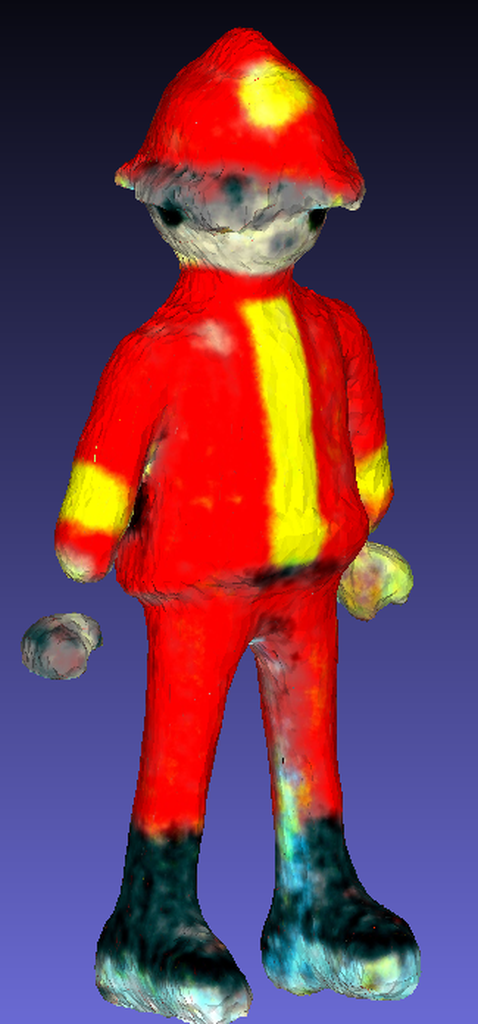
\includegraphics[width=\textwidth]{etc/a high quality rendering of a playmobil firefighter/dreamfusion/dreamfusion_playmobil_result_resize.png}
        \caption{DreamFusion}
    \end{subfigure}
    \begin{subfigure}[b]{0.179\textwidth}
        \centering
        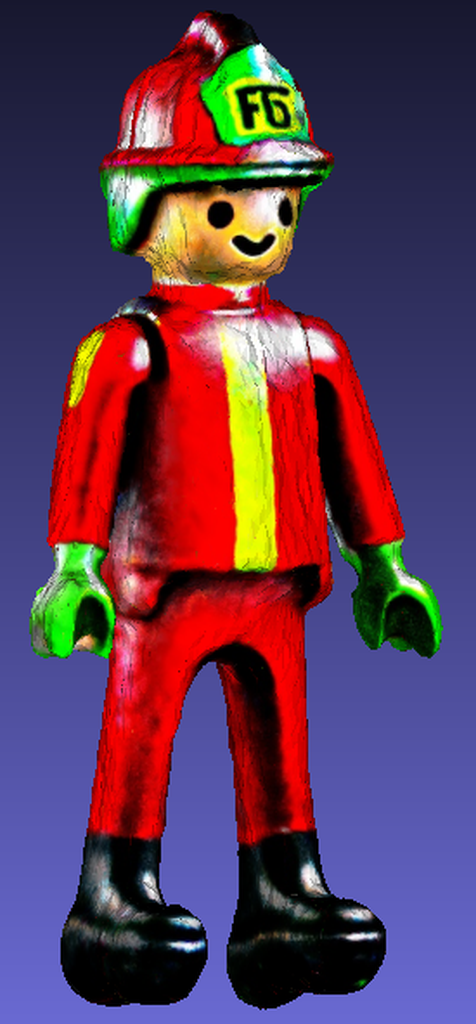
\includegraphics[width=\textwidth]{etc/a high quality rendering of a playmobil firefighter/magic3d/magic3d_playmobil_result_resize.png}
        \caption{Magic3D}
    \end{subfigure}
    \begin{subfigure}[b]{0.227\textwidth}
        \centering
        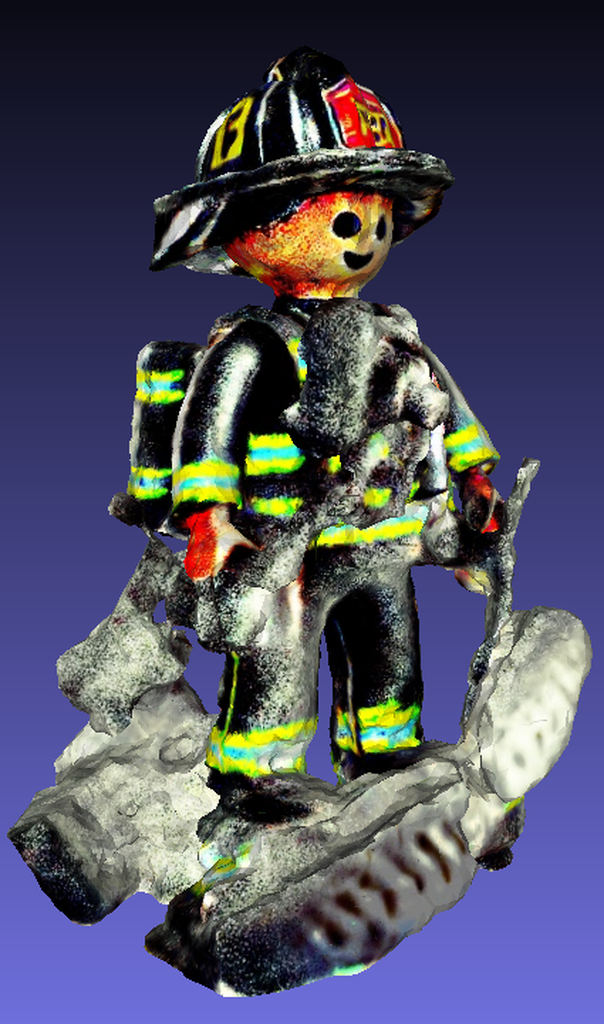
\includegraphics[width=\textwidth]{etc/a high quality rendering of a playmobil firefighter/fantasia3d_Magic3DInput/fantasia_playmobil_result_resize.png}
        \caption{Fantasta3D}
    \end{subfigure}
    \begin{subfigure}[b]{0.192\textwidth}
        \centering
        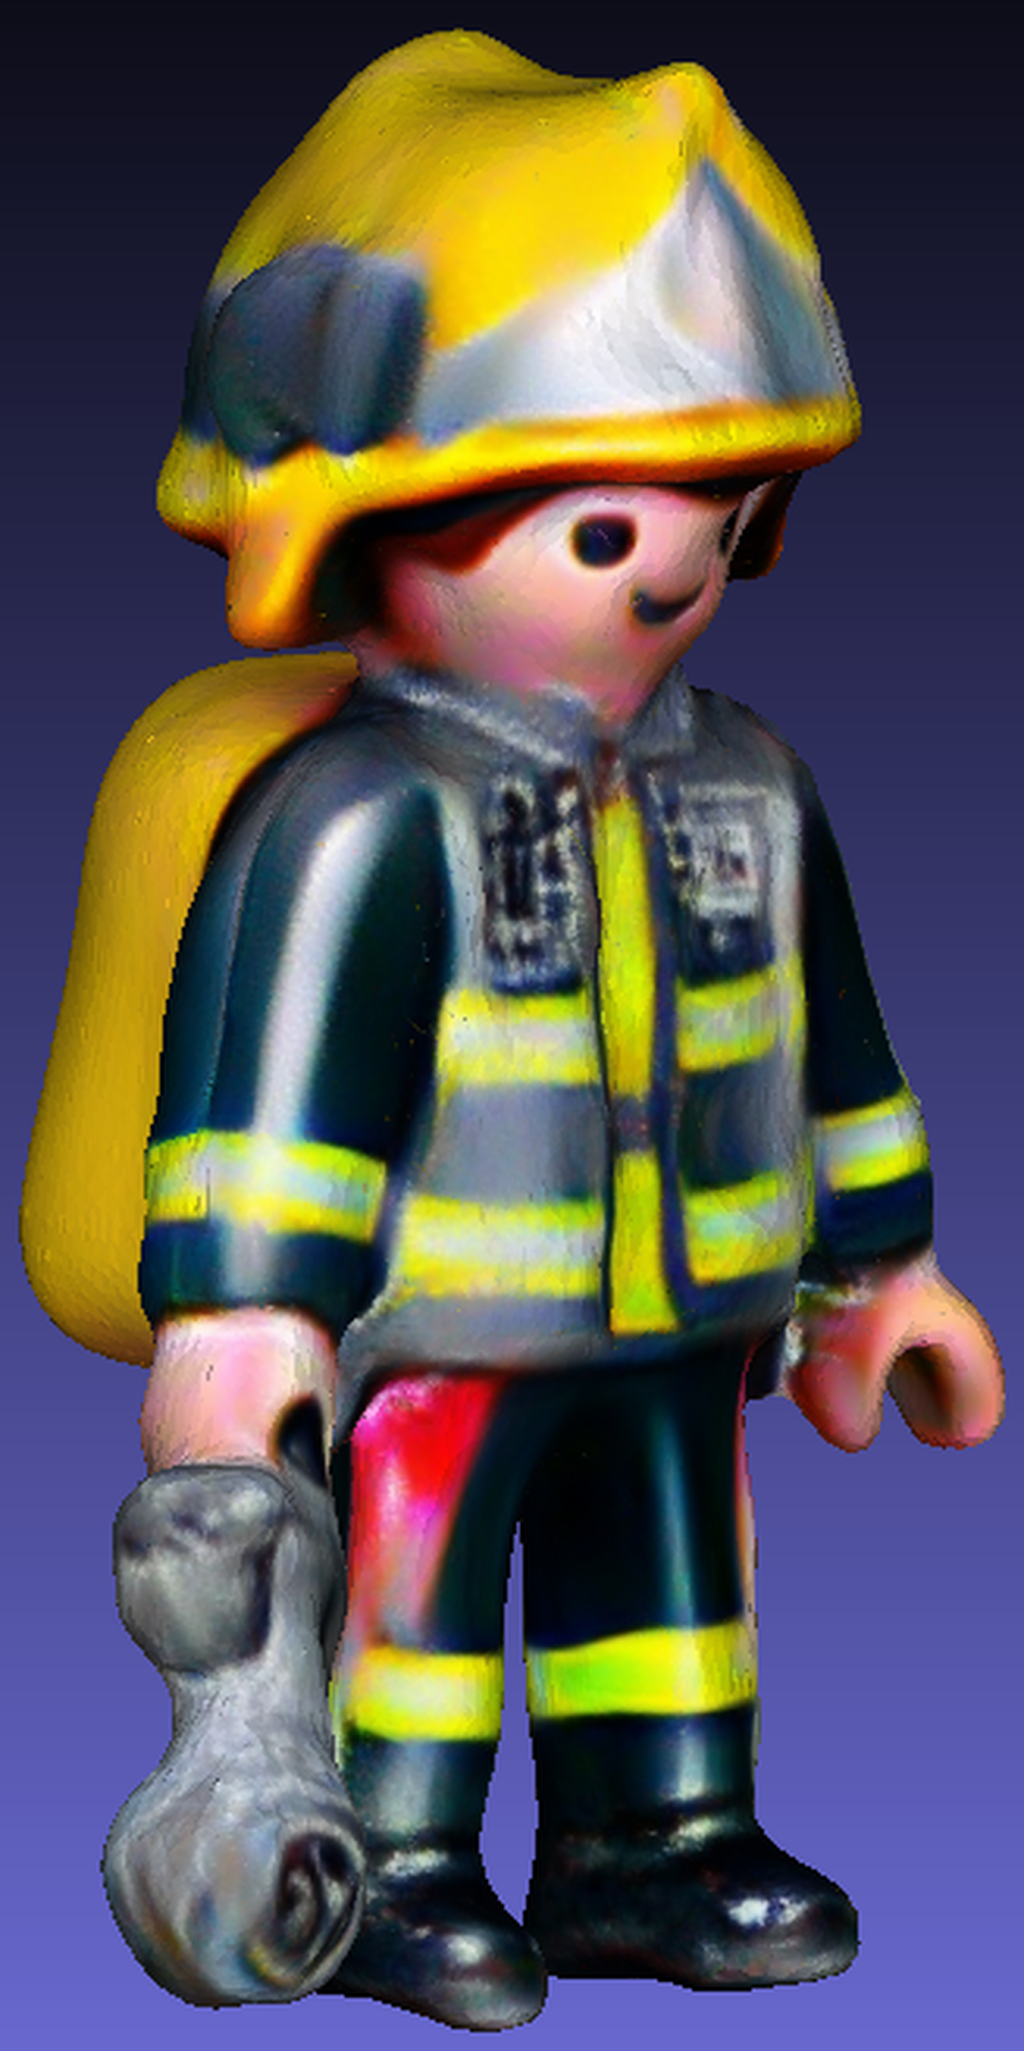
\includegraphics[width=\textwidth]{etc/a high quality rendering of a playmobil firefighter/magic123/magic123_playmobil_result_resize.png}
        \caption{Magic123}
    \end{subfigure}
    \begin{subfigure}[b]{0.181\textwidth}
        \centering
        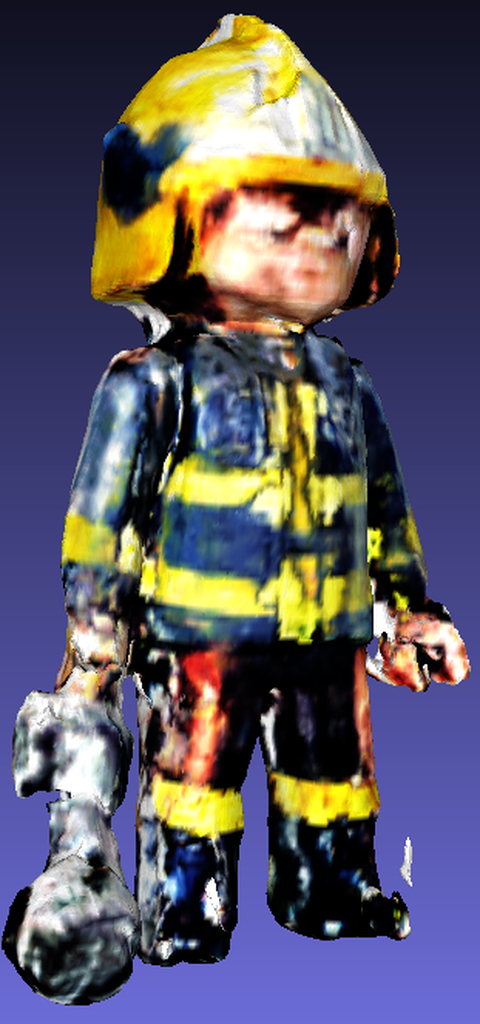
\includegraphics[width=\textwidth]{etc/a high quality rendering of a playmobil firefighter/wonder3D/wonder3d_playmobil_result_resize.png}
        \caption{Wonder3D}
    \end{subfigure}
    \caption{Results obtained using the prompt ``a high-quality rendering of a Playmobil firefighter''.}~\label{fig:resultPlaymobil}
\end{figure}

\textbf{Geometry:} The geometric shape of the models varies significantly. DreamFusion and Wonder3D present the most deviations from the expected Playmobil figure geometry. Both exhibit overly smooth shapes with ambiguous edges and floating elements, such as the hands in DreamFusion and around the right foot in Wonder3D, giving an unfinished appearance. In contrast, Fantasta3D achieves a promising silhouette but includes unintended additional objects, like a presumed fire extinguisher on the back and an ambiguous `thing' at the front, possibly an attempt at rendering a fire hose. Magic123, while delivering a solid representation, introduces a large bag on the figure's back, which, unlike the extraneous parts of Fantasta3D, integrates well with the overall model. A closer look of this bag is given in Figure~\ref{fig:inputPlaymobil} parts (b) and (c). Uniquely, Magic123 recreates the iconic Playmobil hand structure, complete with thumb, fingers, and the characteristic gap between them, capturing the essence of the figure's appendages. In addition, this method impresses with a near-perfect rendering of the Playmobil figure, capturing the sharp transitions at the joints and maintaining smoothness elsewhere, except for a slight distortion around the feet. This result seems like one could bend and move it like it is possible with an original figure.

\textbf{Texture Realism:} In terms of texture, Magic3D again stands out with a level of realism that surpasses the others for the Playmobil prompt. It boasts clear demarcation between the colors, such as the black of the shoes against the red of the uniform, and the face retains the characteristic Playmobil look. The model's interaction with light, evidenced by chest reflections and leg shadows, adds to the plastic appearance. DreamFusion's model lacks such light interplay, resulting in a flat appearance, which is also caused due to the overall smoothened geometry. Fantasta3D, Magic123, and Wonder3D diverge from the red texture, opting for a black and yellow combination with realistic reflective stripes. Fantasta3D's texture is commendable despite some geometric artifacts, with light reflection indicating a clear light source and giving the helmet a metallic sheen. Magic123 captures a plastic-like sheen, particularly on the arm's reflection, which underscores the roundness and smoothness of the figure. In contrast, Wonder3D's texture is disappointingly detailed, blurring distinctions like the separation between jacket and shirt, and failing to render the character's face, similar to DreamFusion. The whole model looks strange, decayed and unfinished.

\begin{figure}[ht]
    \centering
    \small
    \begin{subfigure}[b]{0.25\textwidth}
        \centering
        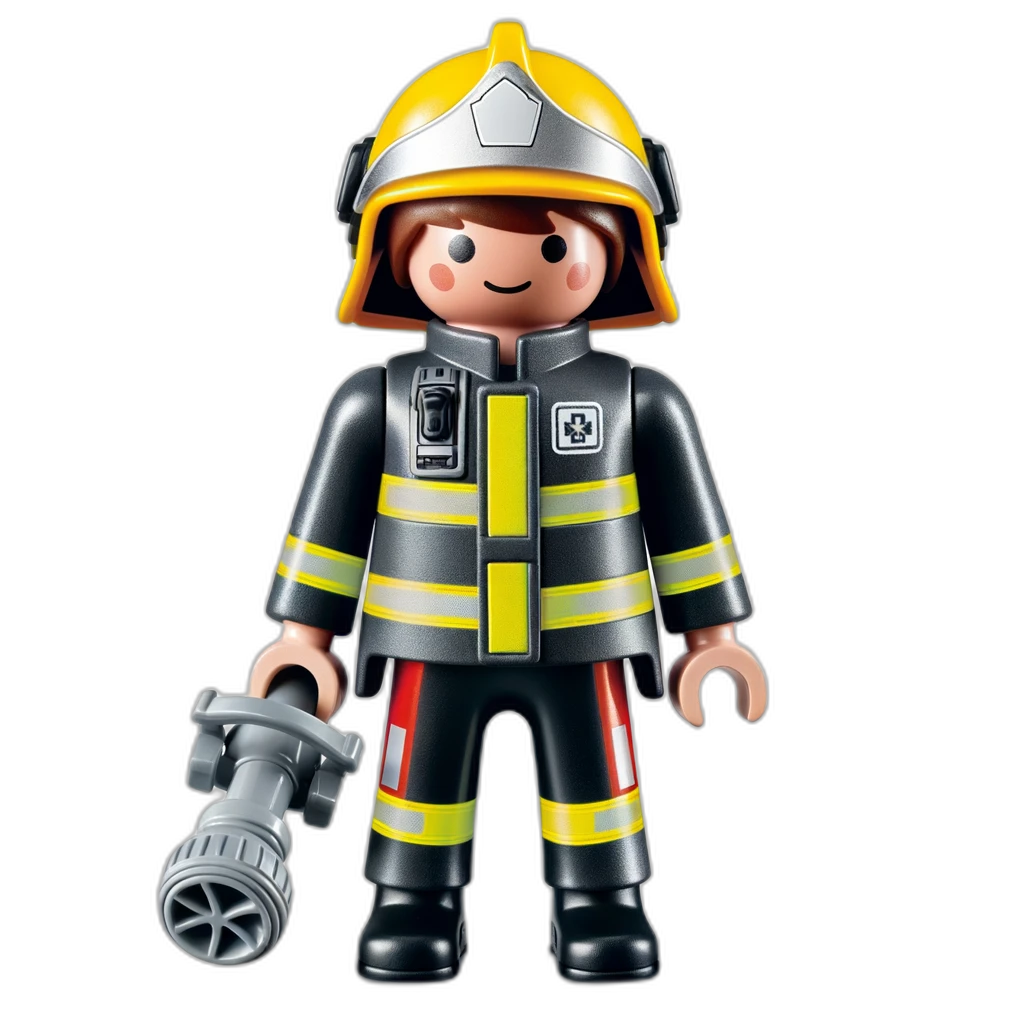
\includegraphics[width=\textwidth]{etc/Images/playmobil.png}
        \caption{}
    \end{subfigure}
    \begin{subfigure}[b]{0.25\textwidth}
        \centering
        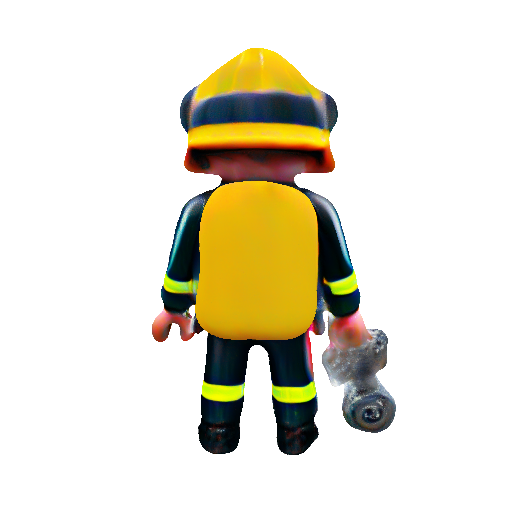
\includegraphics[width=\textwidth]{etc/a high quality rendering of a playmobil firefighter/magic123/magic123_playmobil_refine_back_10000_part1.png}
        \caption{}
    \end{subfigure}
    \begin{subfigure}[b]{0.25\textwidth}
        \centering
        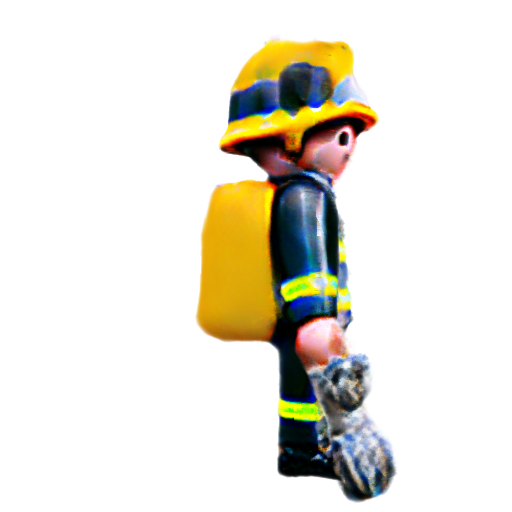
\includegraphics[width=\textwidth]{etc/a high quality rendering of a playmobil firefighter/magic123/magic123_playmobil_coarse_right_10000_part1.png}
        \caption{}
    \end{subfigure}
    \caption{(a) displays the original image for the playmobil figure derived form Dall-E 3; (b and c) show the side and back view of Magic123, resectively}~\label{fig:inputPlaymobil}
\end{figure}

The effectiveness of Evaluate3D is further enhanced by the integration of OpenAI's CLIP-score, a metric that quantifies the correspondence between an image and a given prompt \citep{radfordCLIP}. This is achieved by encoding both the prompt and the image into high-dimensional vectors within the same embedding space, and then determining the cosine similarity between these vectors. Cosine similarity is a measure of orientation rather than magnitude, with the cosine of the angle between two vectors indicating how closely the content of the image mirrors that of the text prompt. Despite its sophisticated design, this score is not without limitations and at times cannot rival the discerning capabilities of the human eye, occasionally leading to outcomes that may seem counterintuitive.

For convenience and to streamline the evaluation process, portions of the code facilitating this metric have been integrated into Evaluate3D. This allows for an immediate calculation of the CLIP-score post-rendering. Utilizing this feature, scores for the Playmobil figures have been computed and are presented in table~\ref{table:scorePlaymobil}. In an intriguing turn, Magic123 ranks highest when assessed against the original prompt, followed by Fantasia3D, Wonder3D, DreamFusion, and finally, Magic3D. These findings are not entirely in concordance with the subjective analysis provided earlier. However, when the prompt is modified to ``a high-quality rendering of a red Playmobil firefighter'', there is a marked reversal in scores. This suggests that the CLIP-score may exhibit a bias towards the color black in the context of firefighter apparel, as opposed to the more toy-like red. The discrepancies highlighted by the CLIP-score accentuate the need for the development of new, more precise evaluation metrics tailored for assessing the output of 3D generative AI, as there currently exists no standard method that is universally recognized as reliable.

\begin{table}[h]
    \centering
    \small
    \begin{tabular}{lccccc}
    \toprule
    Prompt & DreamFusion & Magic3D & Fantasia3D & Magic123 & Wonder3D \\
    \midrule
    a Playmobil firefighter & 0.337 & 0.320 & 0.503 & 0.827 & 0.482 \\
    a red Playmobil firefighter & 0.501 & 0.604 & 0 & 0 & 0.216 \\
    \bottomrule
    \end{tabular}
    \caption{CLIP-scores for Playmobil firefighter models based on different prompts.}~\label{table:scorePlaymobil}
\end{table}
 
The next prompt used for the various methods was ``a rendering of a highly symmetrical loaf of bread''. Using this prompt, the goal was to assess on how close a Method can achieve such specific details in a prompt why still creating some reasonable results. The models generated can be seen in Figure~\ref{fig:resultBread} including not only the resuls but also the generated input image of Dall-E 3 given in part (f). In order to evaluate the symmetrical properties of each models, Evaluate3D is used which incorporates a function from trimesh which effectively mirrors a model along an axes and determines if on the mirrored vertex side exists a vertex, meaning that for this specific point, the model is symmetrical. This is done for all vertrtexes and a score is derived from the amount of counterparts found along an axis. The results of this assemeent can be seen in Table~\ref{table:symmetrieBread}. 

\begin{table}[ht]
    \centering
    \small
    \begin{tabular}{lccccc}
    \toprule
    {} & DreamFusion & Magic3D & Fantasia3D & Magic123 & Wonder3D \\
    \midrule
    Symmetrie Score & 0.337 & 0.320 & 0.503 & 0.827 & 0.482 \\
    \bottomrule
    \end{tabular}
    \caption{Symmetrie-scores for bread models demanding a symmetrical output.}~\label{table:symmetrieBread}
\end{table}

In terms of Prompt/Result Fidelity, only some of results derived here all seem to capture the essence of a bread. The methods in resulting in good bread models are Magic123 and Magic3D. Wonder3D alows to breifly imagine a loaf of bread. DreamFusion and Fantasia3D, however, fall short on this task. The result presented in DreamFusion is only a clubm of anything. The generated model could be clay or a stone or anything else. Fantasia3D's result looks more like a pineapple or some sort of explosion, if no context is given.  

\begin{figure}[ht]
    \centering
    \small
    \begin{subfigure}[b]{0.31\textwidth}
        \centering
        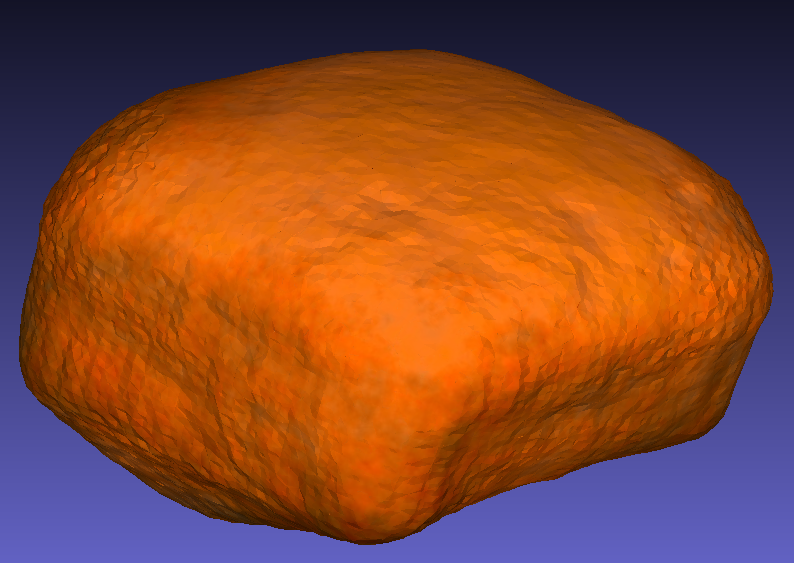
\includegraphics[width=\textwidth]{etc/a rendering of a highly symmetrical loaf of bread/dreamfusion/dreamfusion_bread_result.png}
        \caption{DreamFusion}
        \vspace{0.1cm}
    \end{subfigure}
    \begin{subfigure}[b]{0.31\textwidth}
        \centering
        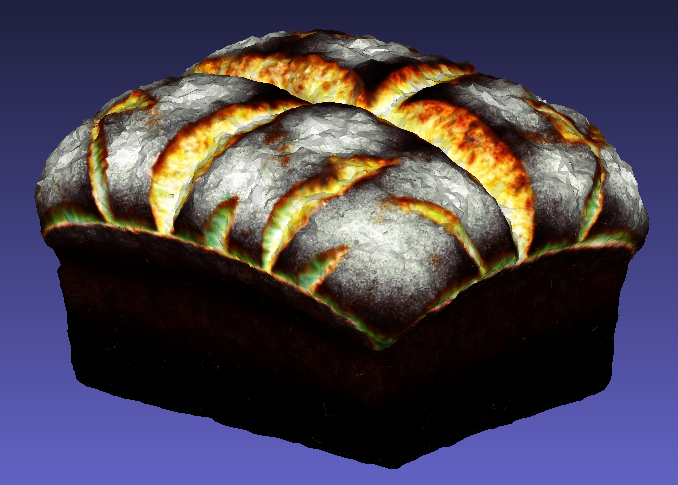
\includegraphics[width=\textwidth]{etc/a rendering of a highly symmetrical loaf of bread/magic3d/magic3D_bread_result.png}
        \caption{Magic3D}
        \vspace{0.1cm}
    \end{subfigure}
    \begin{subfigure}[b]{0.2\textwidth}
        \centering
        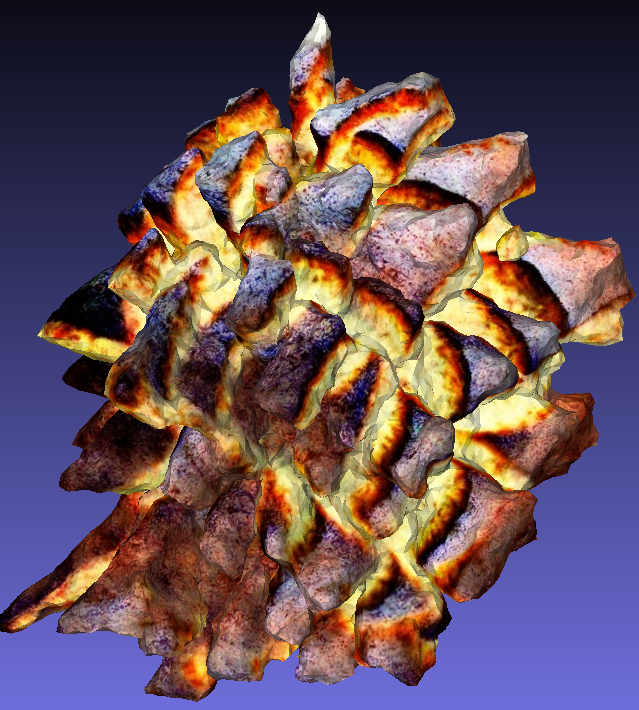
\includegraphics[width=\textwidth]{etc/a rendering of a highly symmetrical loaf of bread/fantasia3d/fantasia_bread_result.png}
        \caption{Fantasta3D}
        \vspace{0.1cm}
    \end{subfigure}

    \begin{subfigure}[b]{0.269\textwidth}
        \centering
        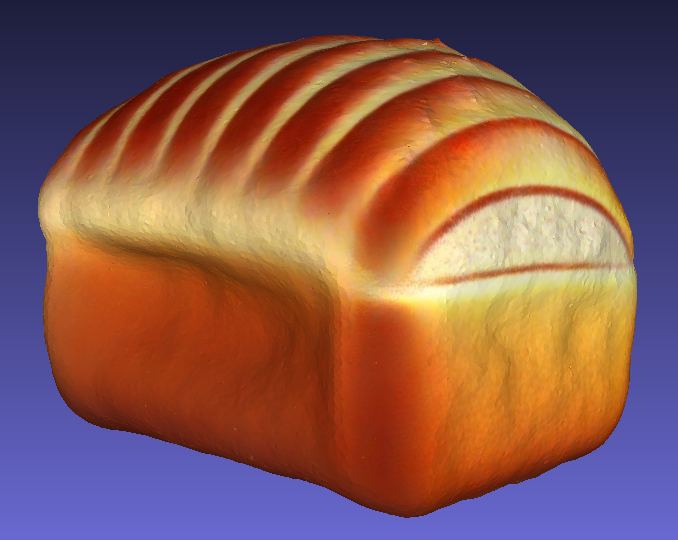
\includegraphics[width=\textwidth]{etc/a rendering of a highly symmetrical loaf of bread/magic123/magic123_bread_result.png}
        \caption{Magic123}
        \vspace{0.1cm}
    \end{subfigure}
    \begin{subfigure}[b]{0.23\textwidth}
        \centering
        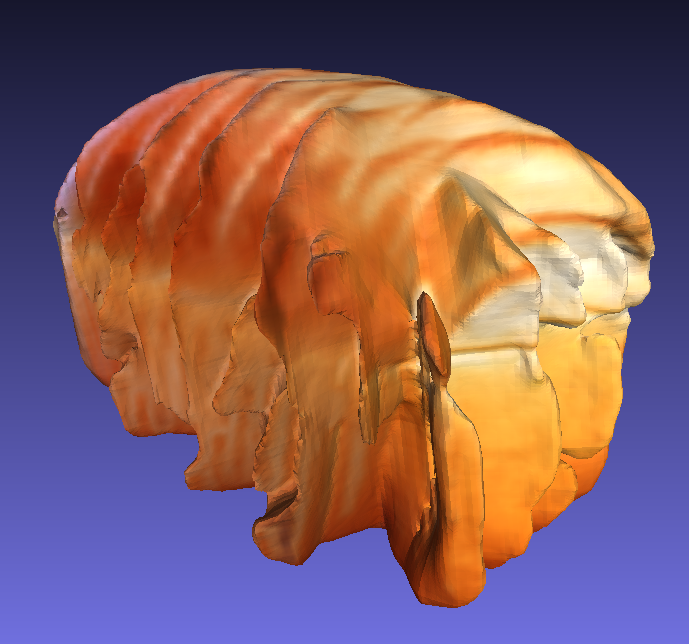
\includegraphics[width=\textwidth]{etc/a rendering of a highly symmetrical loaf of bread/wonder3D/wonder3d_bread_result.png}
        \caption{Wonder3D}
        \vspace{0.1cm}
    \end{subfigure}
    \begin{subfigure}[b]{0.23\textwidth}
        \centering
        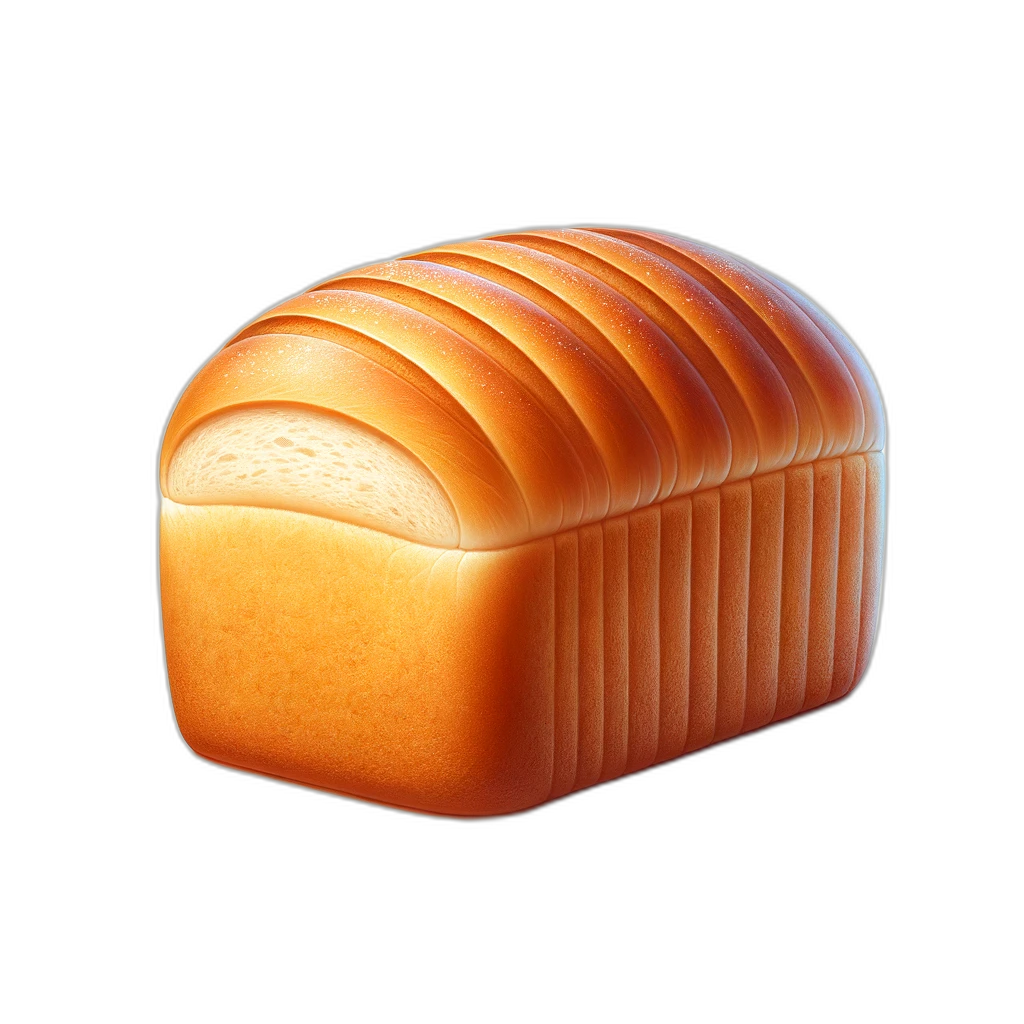
\includegraphics[width=\textwidth]{etc/Images/bread.png}
        \caption{Original Image}
        \vspace{0.1cm}
    \end{subfigure}
    \caption{Results obtained using the prompt ``a rendering of a highly symmetrical loaf of bread''. Part (f) is the input image for Magic123 and Wonder3D, generated with Dall-E 3}~\label{fig:resultBread}
\end{figure}

Geometry: As already mentioned, DreamFusion does not result in anythign meaningful, also including any good geometry. Magic3D, however, achieved generating a model of a bread. The geometry per se does look good, additionaly, the top of the bread does looked carved in, resembling some fresh black bread. Fantasia3D has a spikey result, it seems that the Model did not find a good starting point in order to determine the flat bottom side of a bread, instead it spread accors every view. A reason for thsi could be overfitting or the model being unable to find a starting point. Magic123 generated the best geometerie of a bread, which replicated the input image quite well. The cuts on top match the image, as well as the overall shape. The quadratic body and the halfcircle on top, resembling a good loaf of bread.Wonder3D seems to have the same result as Fantasia3D. a rough shape of a bread is determinable, however, this shape is also kind of spikey towards its sides and the bottom. It seems like Wonder3D did not find a proper way in order to optimize for generating better results. Another reason for the spikey looks of Fantasia3D and Wonder3D are the small changes done to the model while generating a 3D mesh. Changing the input to another output always leads to some sort of error, this could be the case here aswell-

Texture Realism: In my opiniion, the only texture of matter here are the ones from Magic3D, Fantasia3D and Magic123. magic3D's texture looks like a back bread, however, the "body" of the loaf looks a bit burned and dark. The yellow into orange into grey color gradient on top makes the bread look kind of realistic. Only evaluating the colors of Fantasia3D's texture also leads to a good combination of the colors, making the overall result look more like lots of bread sticks are sticked into another. this could only be assessed if some context is given. Magic123 truthfully replicated the original image, showing its ability to generate results that require low detail.


\begin{figure}[ht]
    \centering
    \small
    \begin{subfigure}[b]{0.24\textwidth}
        \centering
        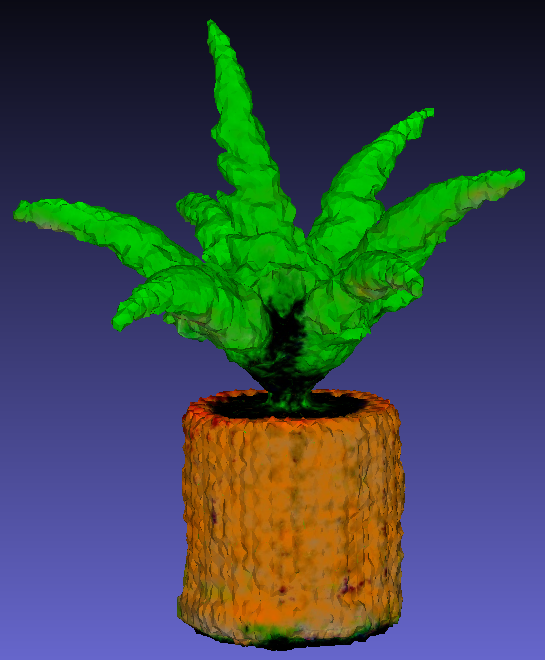
\includegraphics[width=\textwidth]{etc/a high-quality rendering of a fern in a wooden pot/dreamfusion/dreamfusion_fern_result.png}
        \caption{DreamFusion}
        \vspace{0.1cm}
    \end{subfigure}
    \begin{subfigure}[b]{0.35\textwidth}
        \centering
        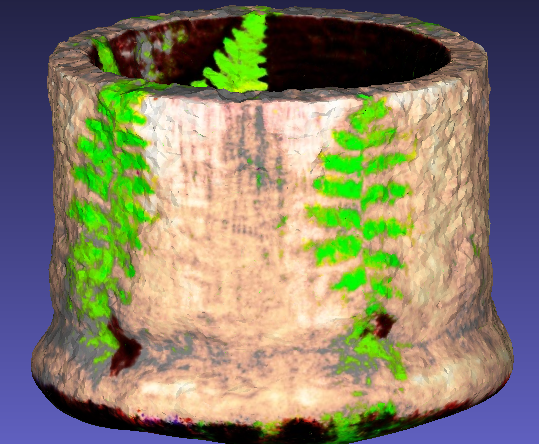
\includegraphics[width=\textwidth]{etc/a high-quality rendering of a fern in a wooden pot/magic3d/magic3d_fern_result.png}
        \caption{Magic3D}
        \vspace{0.1cm}
    \end{subfigure}
    \begin{subfigure}[b]{0.32\textwidth}
        \centering
        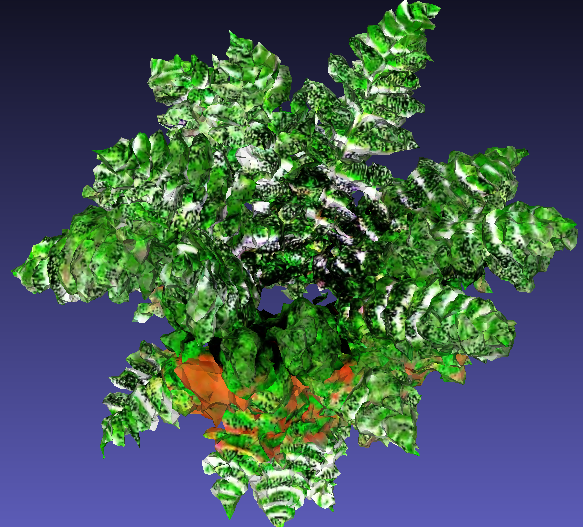
\includegraphics[width=\textwidth]{etc/a high-quality rendering of a fern in a wooden pot/fantasia3d/fantasia_fern_result.png}
        \caption{Fantasta3D}
        \vspace{0.1cm}
    \end{subfigure}

    \begin{subfigure}[b]{0.28\textwidth}
        \centering
        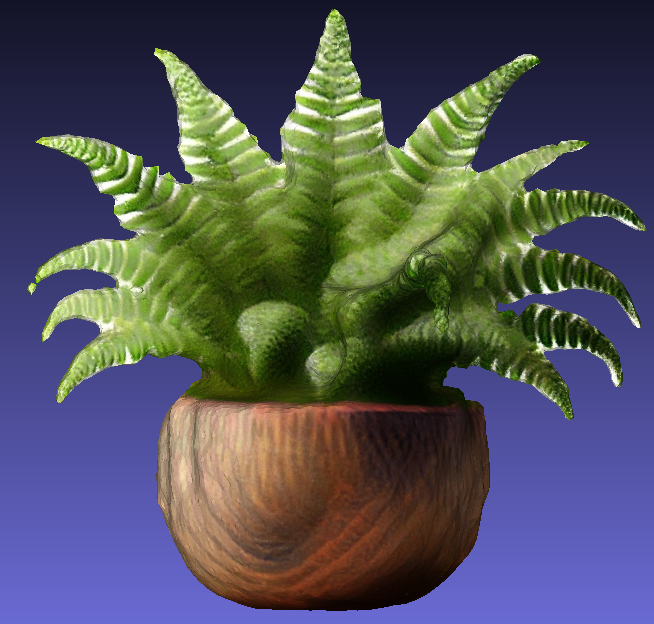
\includegraphics[width=\textwidth]{etc/a high-quality rendering of a fern in a wooden pot/magic123/magic123_fern_front_result.png}
        \caption{Magic123}
        \vspace{0.1cm}
    \end{subfigure}
    \begin{subfigure}[b]{0.27\textwidth}
        \centering
        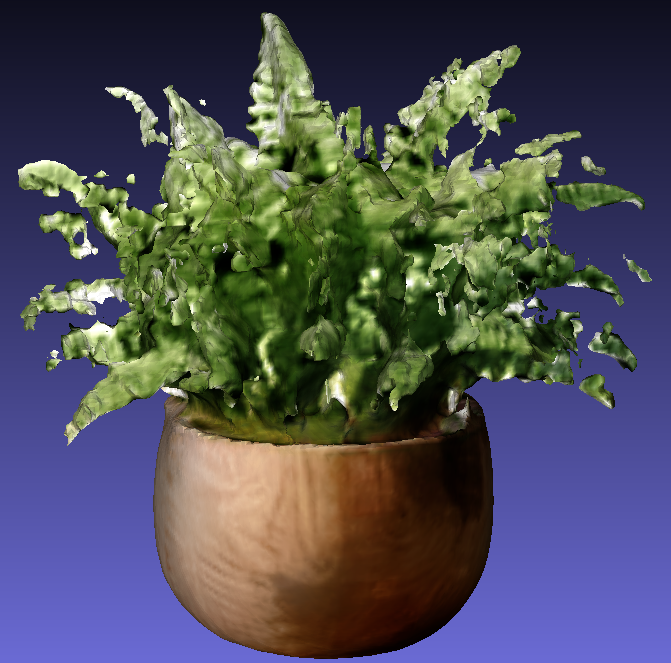
\includegraphics[width=\textwidth]{etc/a high-quality rendering of a fern in a wooden pot/wonder3D/wonder3d_fern_result.png}
        \caption{Wonder3D}
        \vspace{0.1cm}
    \end{subfigure}
    \begin{subfigure}[b]{0.28\textwidth}
        \centering
        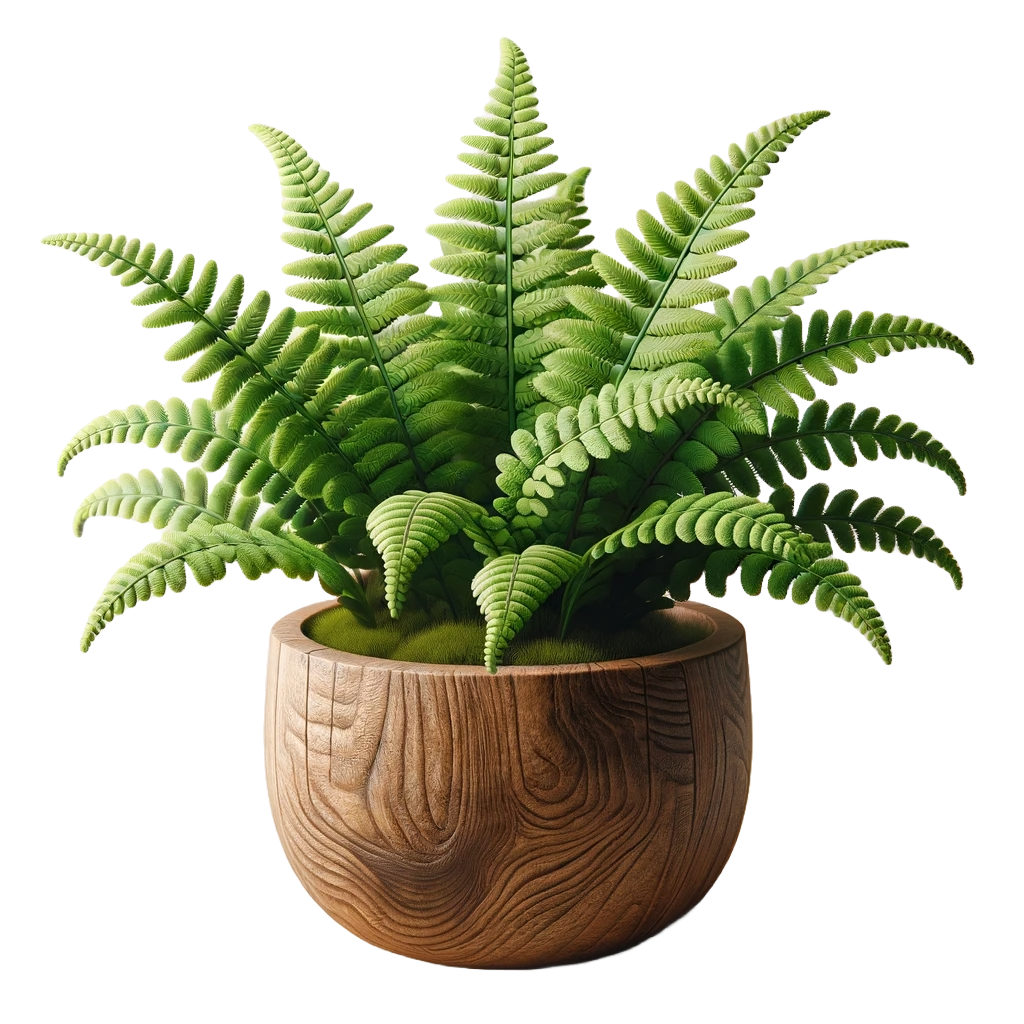
\includegraphics[width=\textwidth]{etc/Images/fern.png}
        \caption{Original Image}
        \vspace{0.1cm}
    \end{subfigure}
    \caption{Results obtained using the prompt ``a high-quality rendering of a fern in a wooden pot''.}~\label{fig:resultFern}
\end{figure}


\begin{figure}[ht]
    \centering
    \begin{subfigure}[b]{0.2\textwidth}
        \centering
        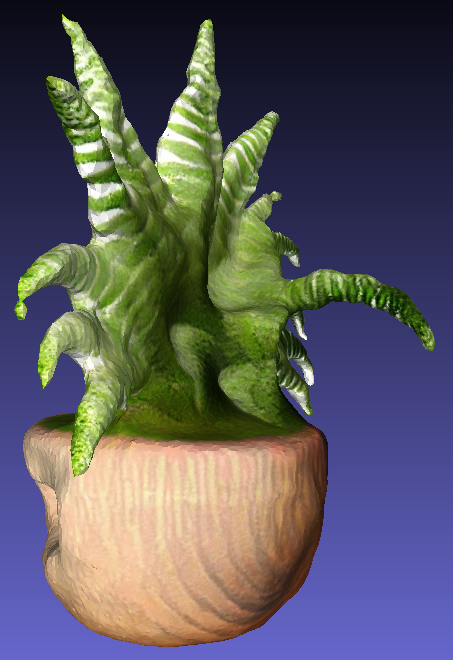
\includegraphics[width=\textwidth]{etc/a high-quality rendering of a fern in a wooden pot/magic123/magic123_fern_side_result.png}
        \caption{Magic123}
    \end{subfigure}
    \begin{subfigure}[b]{0.32\textwidth}
        \centering
        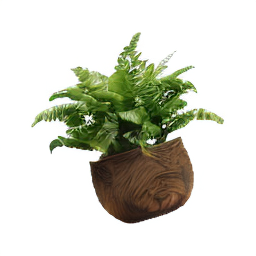
\includegraphics[width=\textwidth]{etc/a high-quality rendering of a fern in a wooden pot/wonder3D/rgb_000_right.png}
        \caption{Wonder3D}
    \end{subfigure}
    \caption{The side view of the fern showcasing the limitations of Magic123 in deriving the correct angles}\label{fig:fernSideview}
  \end{figure}



  \begin{figure}[ht]
    \centering
    \small
    \begin{subfigure}[b]{0.295\textwidth}
        \centering
        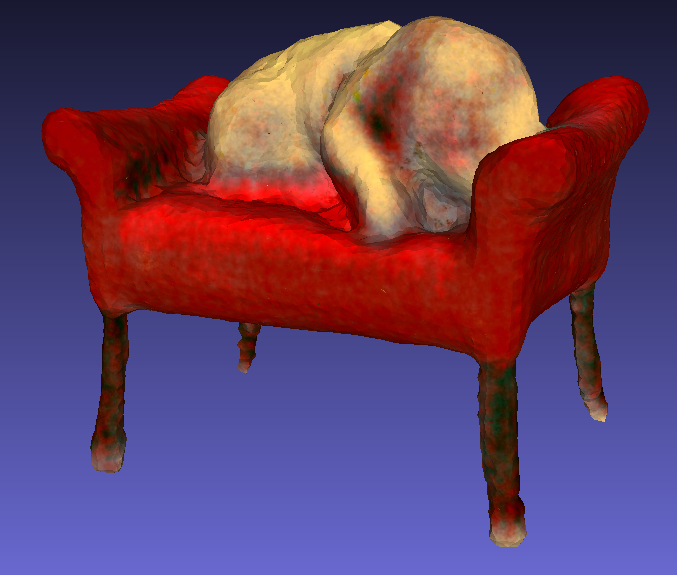
\includegraphics[width=\textwidth]{etc/a high-quality rendering of a big dog sleeping on a chair/dreamfusion/dreamfusion_dog_front_result.png}
        \caption{DreamFusion}
        \vspace{0.1cm}
    \end{subfigure}
    \begin{subfigure}[b]{0.32\textwidth}
        \centering
        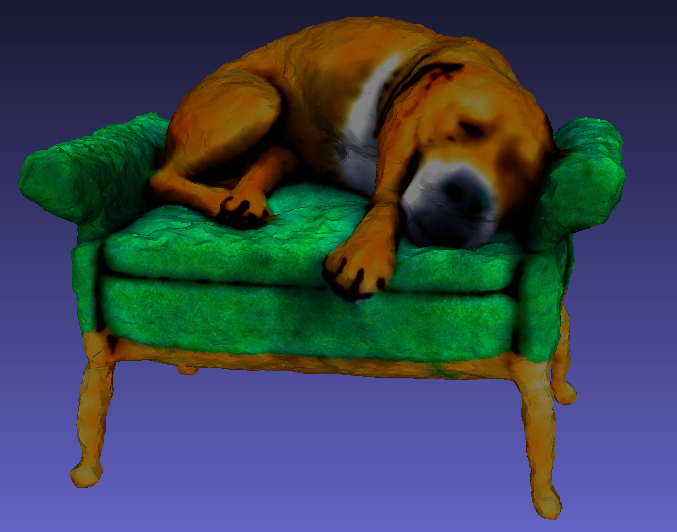
\includegraphics[width=\textwidth]{etc/a high-quality rendering of a big dog sleeping on a chair/magic3d/magic3D_dog_front_result.png}
        \caption{Magic3D}
        \vspace{0.1cm}
    \end{subfigure}
    \begin{subfigure}[b]{0.33\textwidth}
        \centering
        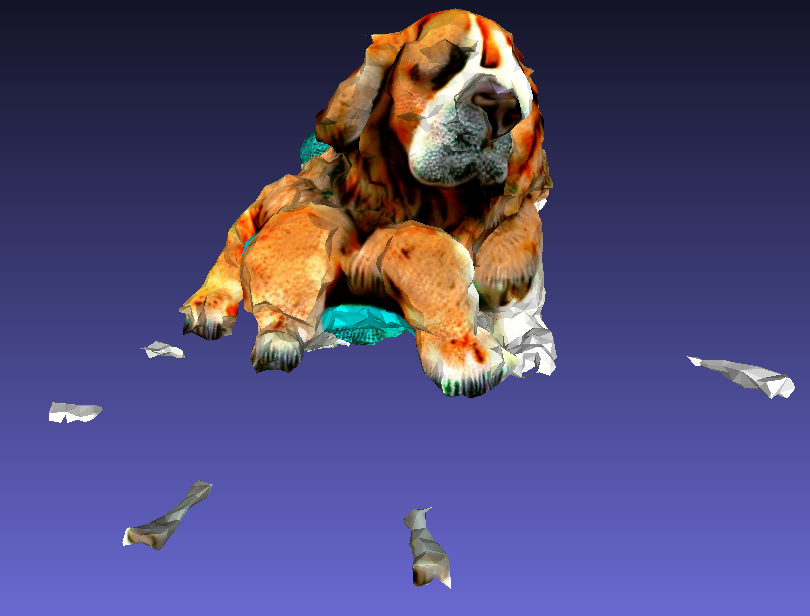
\includegraphics[width=\textwidth]{etc/a high-quality rendering of a big dog sleeping on a chair/fantasia3d/fantasia_dog_front_result.png}
        \caption{Fantasta3D}
        \vspace{0.1cm}
    \end{subfigure}

    \begin{subfigure}[b]{0.267\textwidth}
        \centering
        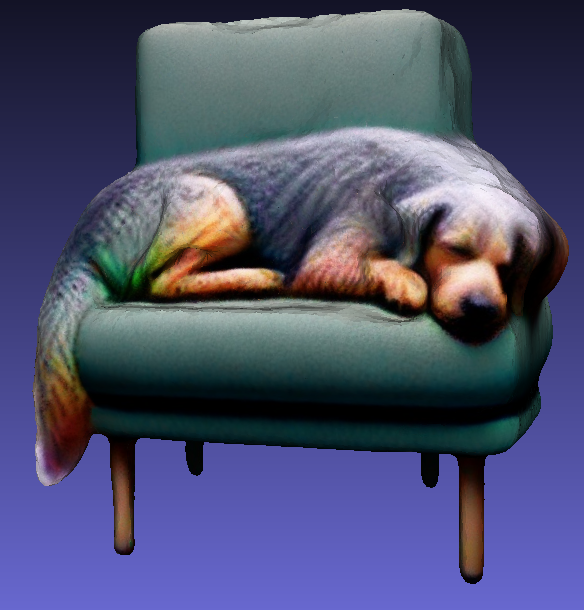
\includegraphics[width=\textwidth]{etc/a high-quality rendering of a big dog sleeping on a chair/magic123/magic123_dog_front_result.png}
        \caption{Magic123}
        \vspace{0.1cm}
    \end{subfigure}
    \begin{subfigure}[b]{0.27\textwidth}
        \centering
        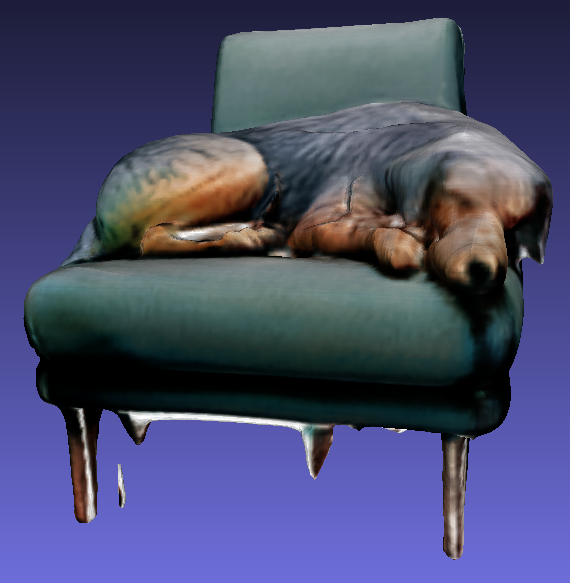
\includegraphics[width=\textwidth]{etc/a high-quality rendering of a big dog sleeping on a chair/wonder3D/wonder3D_dog_front_result.png}
        \caption{Wonder3D}
        \vspace{0.1cm}
    \end{subfigure}
    \begin{subfigure}[b]{0.28\textwidth}
        \centering
        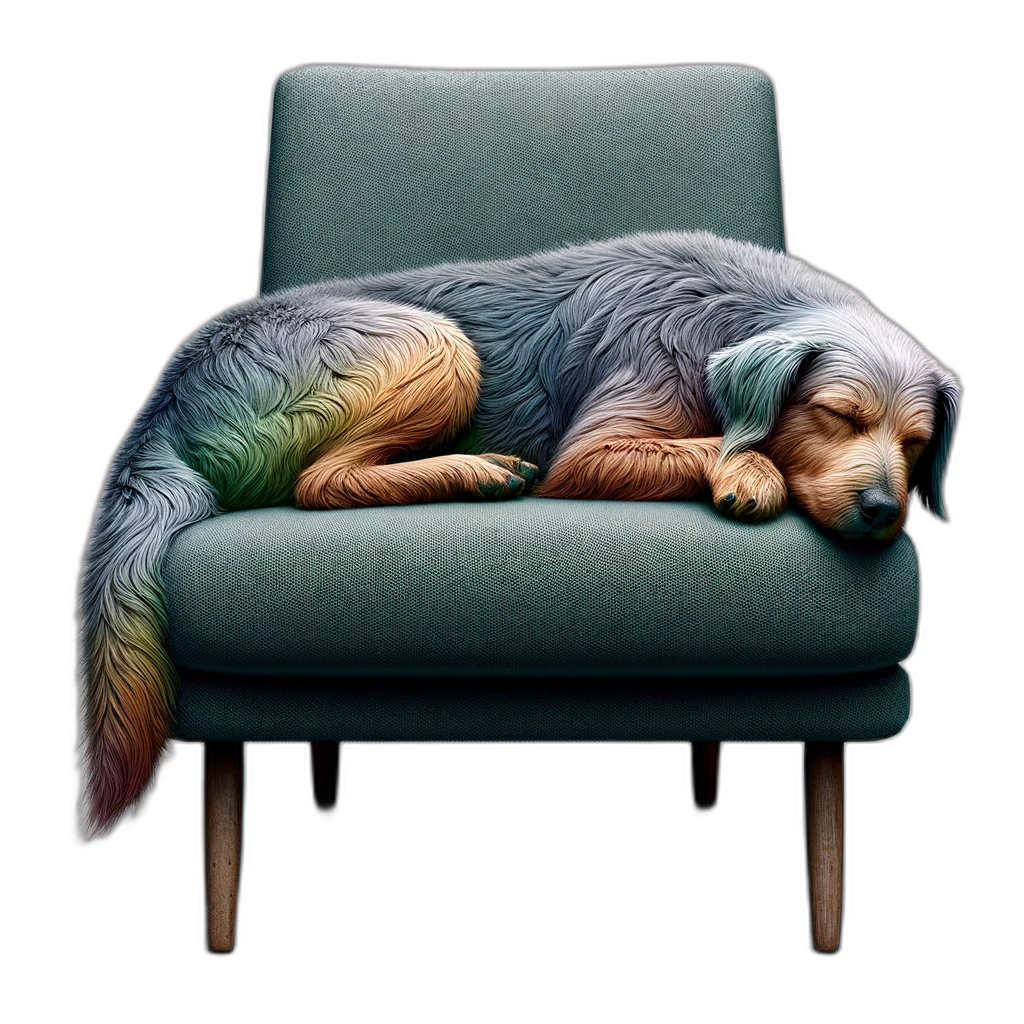
\includegraphics[width=\textwidth]{etc/Images/dog.png}
        \caption{Original Image}
        \vspace{0.1cm}
    \end{subfigure}
    \caption{Results obtained using the prompt ``a high-quality rendering of a big dog sleeping on a chair''.}~\label{fig:resultDogFront}
\end{figure}


\begin{figure}[ht]
    \centering
    \small
    \begin{subfigure}[b]{0.291\textwidth}
        \centering
        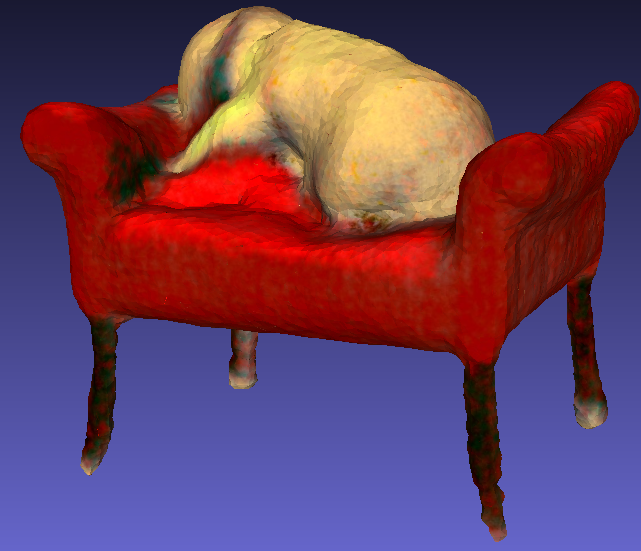
\includegraphics[width=\textwidth]{etc/a high-quality rendering of a big dog sleeping on a chair/dreamfusion/dreamfusion_dog_back_result.png}
        \caption{DreamFusion}
        \vspace{0.1cm}
    \end{subfigure}
    \begin{subfigure}[b]{0.3\textwidth}
        \centering
        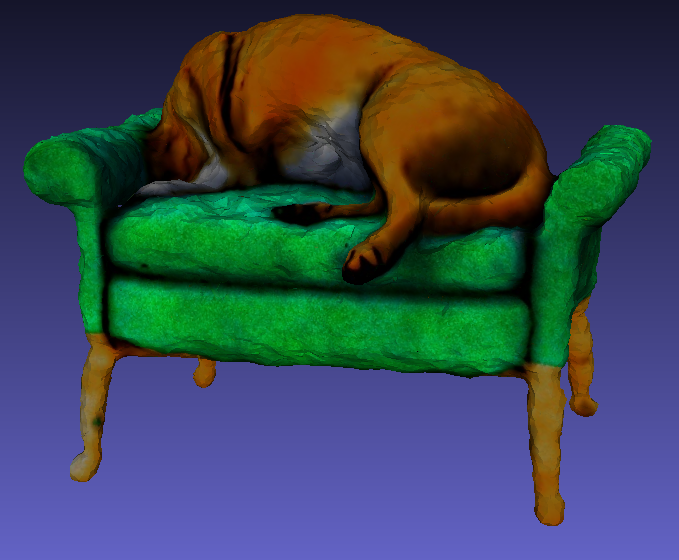
\includegraphics[width=\textwidth]{etc/a high-quality rendering of a big dog sleeping on a chair/magic3d/magic3D_dog_back_result.png}
        \caption{Magic3D}
        \vspace{0.1cm}
    \end{subfigure}
    \begin{subfigure}[b]{0.34\textwidth}
        \centering
        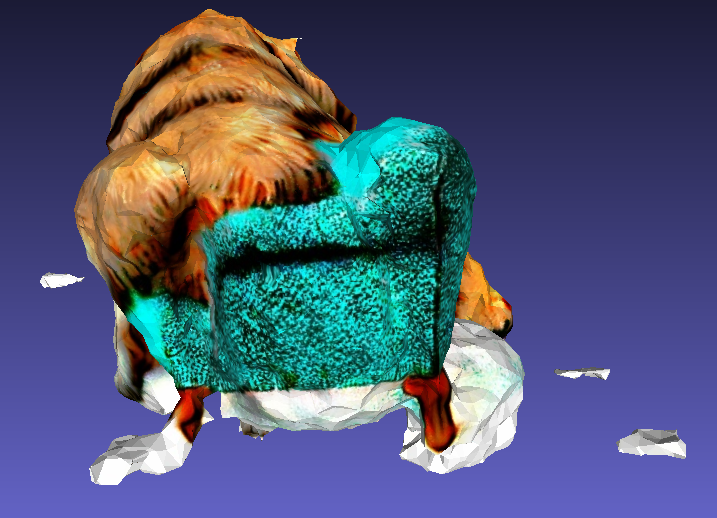
\includegraphics[width=\textwidth]{etc/a high-quality rendering of a big dog sleeping on a chair/fantasia3d/fantasia_dog_back_result.png}
        \caption{Fantasta3D}
        \vspace{0.1cm}
    \end{subfigure}

    \begin{subfigure}[b]{0.261\textwidth}
        \centering
        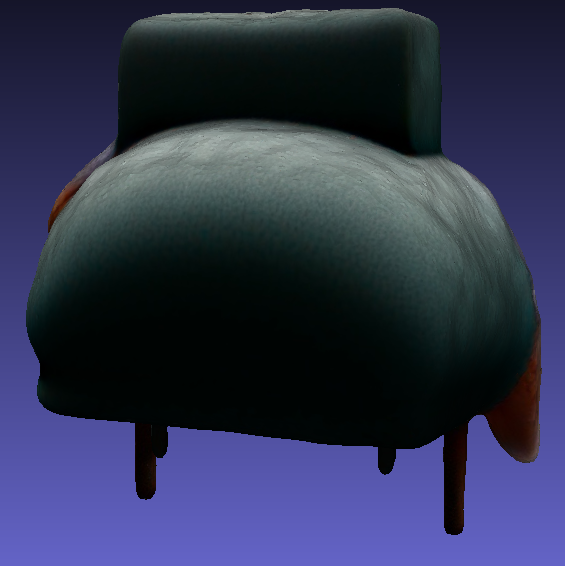
\includegraphics[width=\textwidth]{etc/a high-quality rendering of a big dog sleeping on a chair/magic123/magic123_dog_back_result.png}
        \caption{Magic123}
        \vspace{0.1cm}
    \end{subfigure}
    \begin{subfigure}[b]{0.27\textwidth}
        \centering
        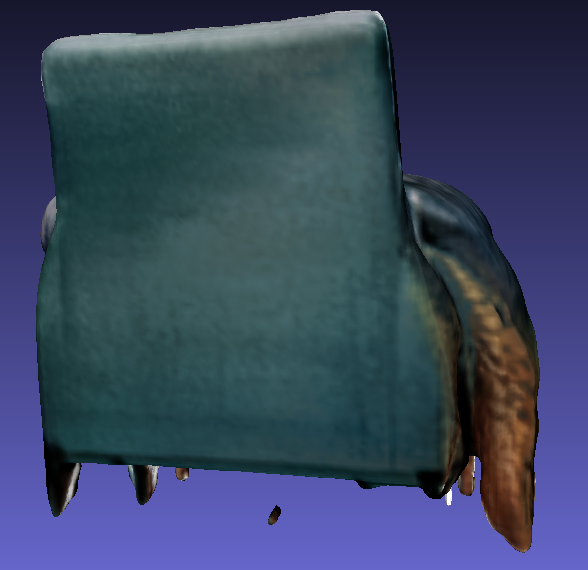
\includegraphics[width=\textwidth]{etc/a high-quality rendering of a big dog sleeping on a chair/wonder3D/wonder3D_dog_back_result.png}
        \caption{Wonder3D}
        \vspace{0.1cm}
    \end{subfigure}
    \caption{Results obtained using the prompt ``a high-quality rendering of a big dog sleeping on a chair''.}~\label{fig:resultDogBack}
\end{figure}


The blow table shows the rendering times required for each prmompt with each model. 

\begin{table}[ht]
    \centering
    \small 
    \begin{tabular}{lcccccccc}
    \toprule
    Prompt & DreamFusion & \multicolumn{2}{c}{Magic3D} & \multicolumn{2}{c}{Fantasia3D} & \multicolumn{2}{c}{Magic123} & Wonder3D \\
    \cmidrule(r){3-4} \cmidrule(lr){5-6} \cmidrule(l){7-8}
    & & \multicolumn{1}{c}{Coarse} & \multicolumn{1}{c}{Refine} & \multicolumn{1}{c}{Geom.} & \multicolumn{1}{c}{Appear.} & \multicolumn{1}{c}{C.} & \multicolumn{1}{c}{R.} &  \\
    \midrule
    Robot & 1:24 & 1:23 & 1:20 & 1:15 & 1:18 & 1:46 & 1:47 & 0:15 \\
    Playmobil & 1:17 & 1:17 & 1:18 & 1:14 & 1:17 & 1:46 & 1:46 & 0:15 \\
    Fern & 1:25 & 1:24 & 1:19 & 1:17 & 1:20 & 1:52 & 1:48 & 0:15 \\
    Bread & 1:25 & 1:21 & 1:21 & 1:17 & 1:20 & 1:54 & 1:52 & 0:15 \\
    \bottomrule
    \end{tabular}
    \caption{Comparison of Generation Times for Different Prompts Across Methods (Hours:Minutes). Legend: C = Coarse, R = Refine, Geom = Geometry, Appear = Appearance.}~\label{table:generation_times_complex}
\end{table}

    
    
    
    